\documentclass[../../Rapport RayTracer]{subfiles}


\begin{document}

Comme présenté dans la section \ref{multithreading}, nous application tire partie de toute la puissnce du processeur de la machine. Le but étant de réduire le temps de calcul, nous présentons dans cette section les gains perçus en terme de performances.\\
Nous comparerons les temps de rendu par image pour différentes résolutions et différents nombre de threads. L'image sera toujours découpée en $nbThread^2$ tuiles.

\begin{figure}[h!]
	\adjustbox{center}{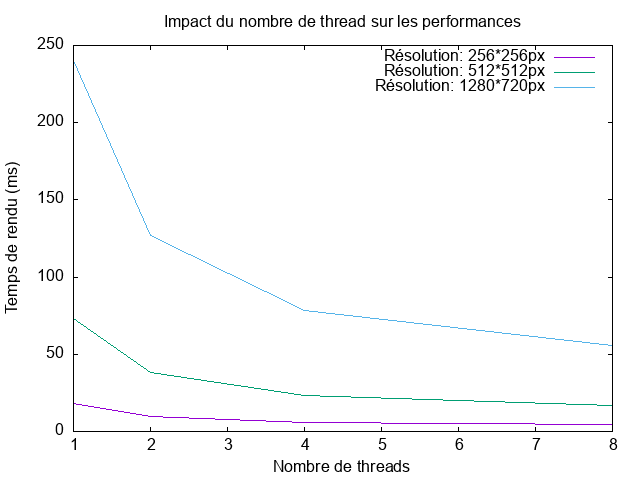
\includegraphics[width=1\textwidth]{img/rt/MultithreadingGraph.png}}
	
	\caption{Graph de l'impact du nombre de thread sur le temps de rendu par image}
	\label{graphMultithreading}
\end{figure}
\FloatBarrier
Toutes les mesures ont été faites sur un CPU disposant de 8 processeurs. La scène rendue est la même que celle de la \figurename\ \ref{reflectionsDemo}.\\
On observe une réduction significative des temps de rendu quand le nombre de threads utilisé augmente. On passe en effet, pour une résolution de 512*512, de 72.87ms en moyenne à 16.72ms de temps de calcul par image. Cela se traduit par un affichage fluide d'un peu moins de 15 images par seconde avec 1 thread. Avec 8 threads, nous passons à environ 60 images par seconde. Les performances ont donc été multipliées par 4.\\
Cette multiplication des performances nous permet entre autre de pouvoir profiter de mouvements fluides lorsque l'on déplace la caméra. Sans ces 8 threads, les mouvement seraient saccadés et peu agréables dû aux temps de rendu trop importants. Bien entendu, les temps de rendu dépendent aussi de la complexité de la scène. Nous avons remarqué que les matériaux réfractifs ont tendance à être plus lourds à calculer que les matériaux mats. Cela s'explique par le fait qu'un matériau réfractif demande de nombreux appels récursifs.

\end{document}